\mode*

\section{Introduction}%
\label{Introduction}

Alice organizes a street protest against Eve's regime.
Bob, Carol and many others participate in the demonstration.
One problem that has not yet been entirely solved is the crowd-counting 
problem, i.e.\ to verify how many participated in Alice's protest.

\mode<presentation>{%
\subsection{What's the problem?}
}

\begin{frame}<presentation>
  \begin{block}{The crowd-counting problem}
    \begin{itemize}
      \item Alice organizes a protest against Eve's regime.
      \item Bob, Carol and others show up.
      \item We want to know how many showed up to support Alice.
    \end{itemize}
  \end{block}
\end{frame}

\mode<presentation>{%
\subsection{Why is it a problem?}
}

\mode<presentation>{%
\begin{frame}
  \begin{figure}
    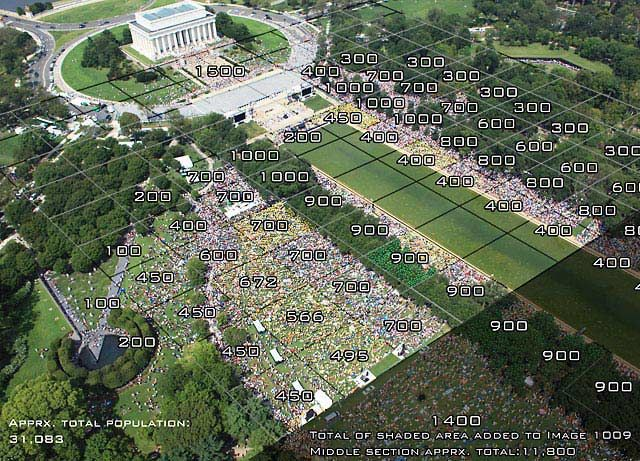
\includegraphics[height=0.9\textheight]{fig/Jacobs-method.jpg}
  \end{figure}
\end{frame}

\begin{frame}
  \begin{example}
    \begin{itemize}
      \item Computer vision does object recognition.
      \item Requires photos/video that cover the entire location, all the time.
      \item This will count people twice.
    \end{itemize}
  \end{example}

  \pause{}

  \begin{example}
    \begin{itemize}
      \item Scan active mobile phones in the area.
      \item This requires some extra equipment.
      \item This catches bystanders who are not protesting.
    \end{itemize}
  \end{example}
\end{frame}
}

\mode<none>{%
\begin{frame}
  \begin{example}
    \begin{itemize}
      \item South Korea 2016~\cite{2016DemonstrationsInSeoul}:
        approximate count by imagery.
        \begin{description}
          \item[Organizers] 1\,000\,000
          \item[Police] 260\,000
        \end{description}

        \pause{}

      \item US 2017~\cite{2017WomensMarchesInUS}:
        sum up people's approximations.
      \item This makes it even difficult to estimate the error.
    \end{itemize}
  \end{example}
\end{frame}
}

After many demonstrations the count by police and that by the organizers 
differ\footnote{%
  This is actually quite natural, they have different goals.
  The organizers want to count everyone who ever participated.
  Police want to estimate the count at the peak of participation, due to crowd 
  control~\cite{2016DemonstrationsInSeoul}.
}, in some instances the difference can be hundreds of thousands.
There are numerous examples, e.g.\ the demonstrations in South 
Korea~\cite{2016DemonstrationsInSeoul}, Trump's 
inauguration~\cite{HowWillWeKnowTrumpInauguralCrowdSize} or the Women's Marches 
in the US~\cite{2017WomensMarchesInUS}, where there is difficulty in 
establishing the actual number of participants.
The methods for counting the crowds vary.
Most of the available methods lack precision, i.e.\ they have large error 
margins.
They can only give an estimate for a particular snapshot in time, e.g.\ at the 
peak of the event, not the cumulative participation count --- at least not 
without counting some people multiple times, which in turn increases the error 
of the estimation.
Finally, they also lack verifiability, i.e.\ everyone must trust the entity who
does the counting.
We will discuss them in more detail in \cref{RelatedWork}.

\begin{frame}<presentation>
  \begin{block}{Verifying protest participation}
    \begin{itemize}
      \item Alice organizes a protest against Eve's regime.
      \item Bob, Carol and others show up.

        \pause{}

      \item {\color{green} Alice wants to show that many support her cause.}

        \pause{}

      \item {\color{red} Eve wants to show that few support Alice's cause.}
      \item It's an adversarial setting!
      \item We need verifiable results.
    \end{itemize}
  \end{block}
\end{frame}

We can make one important observation about this problem that has seemingly 
been ignored in the past: it is an adversarial setting.
The protesters (organizers and participants) have an incentive to increase the 
tallied number of participants, whereas other interests might have an incentive 
to decrease the tallied number of participants, e.g.\ Eve's authoritarian 
regime in our example above.
Or the other way around, sometimes Eve's authoritarian regime wants to organize 
a pro-regime protest to demonstrate its \enquote{wide 
  support}~\cite[e.g.][]{AlJazeeraOnVenezuela2017,VenezuelanStateWorkersCalledToParticipate}.
(This makes it difficult to rely on government-issued credentials to prevent a 
Sybil attack --- government can issue arbitrarily many such credentials for its 
own protests.)
To solve this problem, we need a verifiable participation count which is 
protected from Sybil attacks.

\mode<article>{%
\subsection{Contributions}
}

In this paper, we combine the verifiability and privacy properties of 
electronic voting with location-proof systems to provide a verifiable 
participation count.
We can only provide a verifiable participation count for non-government 
protests:
In any pro-government protest we cannot prevent the government from doing a 
Sybil attack, since the government controls the identity system.

%In the case of the Korean demonstrations~\cite{2016DemonstrationsInSeoul}, this 
%was in one place during an entire day and then repeated for several weekends.
%In the case of the Women's Marches in the US~\cite{2017WomensMarchesInUS}, they
%were in several locations at the same time.

%\blockcquote{HowToEstimateCrowdSize}{%
%  Crowd size is also needed for media news reports and to historically record 
%  the event%
%}

